\documentclass[10pt]{sig-alternate}
\makeatletter
\def\@copyrightspace{\relax}
\makeatother

\usepackage{hyperref}
\usepackage{listings}

\newcommand{\quotes}[1]{``{#1}''}

\usepackage{xcolor}

\colorlet{punct}{red!60!black}
\definecolor{background}{HTML}{EEEEEE}
\definecolor{delim}{RGB}{20,105,176}
\colorlet{numb}{magenta!60!black}

% There is no lst-language highlighting json code nicely. Hence, we define it here.
\lstdefinelanguage{json}{
    basicstyle=\normalfont\ttfamily,
    numbers=left,
    numberstyle=\scriptsize,
    stepnumber=1,
    numbersep=8pt,
    showstringspaces=false,
    breaklines=true,
    frame=lines,
    backgroundcolor=\color{background},
    literate=
     *{0}{{{\color{numb}0}}}{1}
      {1}{{{\color{numb}1}}}{1}
      {2}{{{\color{numb}2}}}{1}
      {3}{{{\color{numb}3}}}{1}
      {4}{{{\color{numb}4}}}{1}
      {5}{{{\color{numb}5}}}{1}
      {6}{{{\color{numb}6}}}{1}
      {7}{{{\color{numb}7}}}{1}
      {8}{{{\color{numb}8}}}{1}
      {9}{{{\color{numb}9}}}{1}
      {:}{{{\color{punct}{:}}}}{1}
      {,}{{{\color{punct}{,}}}}{1}
      {\{}{{{\color{delim}{\{}}}}{1}
      {\}}{{{\color{delim}{\}}}}}{1}
      {[}{{{\color{delim}{[}}}}{1}
      {]}{{{\color{delim}{]}}}}{1},
}



\begin{document}

% Copyright
\setcopyright{acmcopyright}

\title{
  % 
\includegraphics[width=0.2\textwidth]{hpi_logo_2017}\\
  \vspace{24pt}
  % In-Memory Trajectory Analysis on Taxi Data
  Comparison of Different Data Layouts for Columnar In-Memory Databases on the Basis of an Example Application
}
\subtitle{
  Seminar Trends and Concepts 3\\
  Summer Semester 2018
}

\numberofauthors{3}

\author{
  Marcel Jankrift, Sebastian Kliem, Toni Stachewicz\\[12pt]
  Supervisors:\\
  Dr. Matthias Uflacker, Keven Richly
}


\maketitle
\begin{abstract}
The taxi business is an extremely competitive market. Private ridesharing companies such as Uber or Lynx have grown tremendously in the last decade. In order to survive as a traditional taxi company, the drivers have to increase their profit even further. Therefore, we created an application, that analysis taxi data recorded over one day in the city of Shenzhen. We examine which taxis were the most profitable ones by calculating the distances and times driven with a passenger. From this information, we can draw specific recommendations, where to take passengers at a certain time, so that the profit can be maximized.
\end{abstract}

\keywords{Geospatial data, Trajectory analysis, Taxi data, In-Memory}

\section{Motivation}

Storing trajectory data in traditional relational databases is not always the best idea. Requests might take a long time when working on big data sets. It is also difficult to achieve good compression rates. There exist some systems which are purely designed to work with such trajectories. Those systems are performing much better than the traditional databases.

In our project we would like to investiage how a columnar in-memory database can handle trajectory data. Thereby, we can make use of the in-memory architecture and of the columnar storage benefits. We developed an example application which covers a lot of real world requests to a large trajectory data set. This application builds a good basis to benchmark different data layouts and optimizations.

Traditional taxi companies like to increase their profit. For that, the individual taxi drivers would have to find many passengers and minimize their waiting times. A way to be a  good performing taxi is to stay in a profitable area of the city. For example, where taxi rides are highly needed at a specific time. With our help, the taxi companies can develop new strategies. A simple strategy would be to only accept and assign orders whose destination is in a good area for the expected arrival time. We created an interactive map, which shows the best performing taxis for one day in Shenzhen. This is based on a data set that is explained in section \ref{sec:ds}. The application has some additional information about the taxi density and numbers about pick-ups and drop-offs. Taxi companies could use the application to quickly analyze the collected GPS data.\\

\section{Data Sources}
\label{sec:ds}

The data we used is a freely available collection of GPS information of taxis.\footnote{\href{https://www-users.cs.umn.edu/~tianhe/BIGDATA/UrbanCPS/TaxiData/TaxiData}{https://www-users.cs.umn.edu/$\sim$tianhe/BIGDATA/\\UrbanCPS/TaxiData/TaxiData}} The dataset set has been collected over one day starting at 12~AM and 23:59~PM in the city of Shenzhen, China and the surrounding area. The data does not only contain the GPS location at a certain time, but also the current speed and the taxi's occupancy. The status of a driving taxi has been recorded in an average interval of 26.85 seconds or every 15 seconds in median. In total there are 14,728 trajectories traced resulting in almost 47 million records. The data comes in CSV-format which can be loaded into the SAP HANA database immediately. One sample point contains six attributes: trajectory id (TID), longitude, latitude, timestamp, speed and a flag indicating the presence of a passenger.

\subsection{Data Cleansing}
Before we started analyzing the trajectories we had a closer look at the dataset itself. We noticed rather soon, that there are some inconsistencies within data. Hence, we perform data cleansing. In the following paragraphs, we describe our criteria for data cleansing in detail.

\subsubsection{Duplicates}
The data was already imported into the database by our supervisor, when we started our project. Since, we did not want to change the the original data we created an own table. Once we wanted to create a primary key, the database has thrown an error stating that the data has duplicate values. In fact, there are 381 data points occuring not only twice, but also multiple times. We deleted those entries, because they do not add any value to the data and prevent the creation of a primary key.

\subsubsection{Bounding box}
Generally, GPS coordinates are not completely accurate. However, there are points in the data set, that do not make sense, are not even possible or do not fit into the geospatial system of longitudes and latidues. The graphic \ref{fig:bbox} below shows the trajectory with id \textit{22,360} which passes through the ocean. In order to eliminate such outliers, we use a bounding box (rectangle highlighted in red color). To avoid deleting points that are outside this area, because there a taxi really drove there, we have chosen the rectangle intentionally large. This data cleansing step effects almost 8,000 GPS points.

\begin{figure}[ht]
\centering
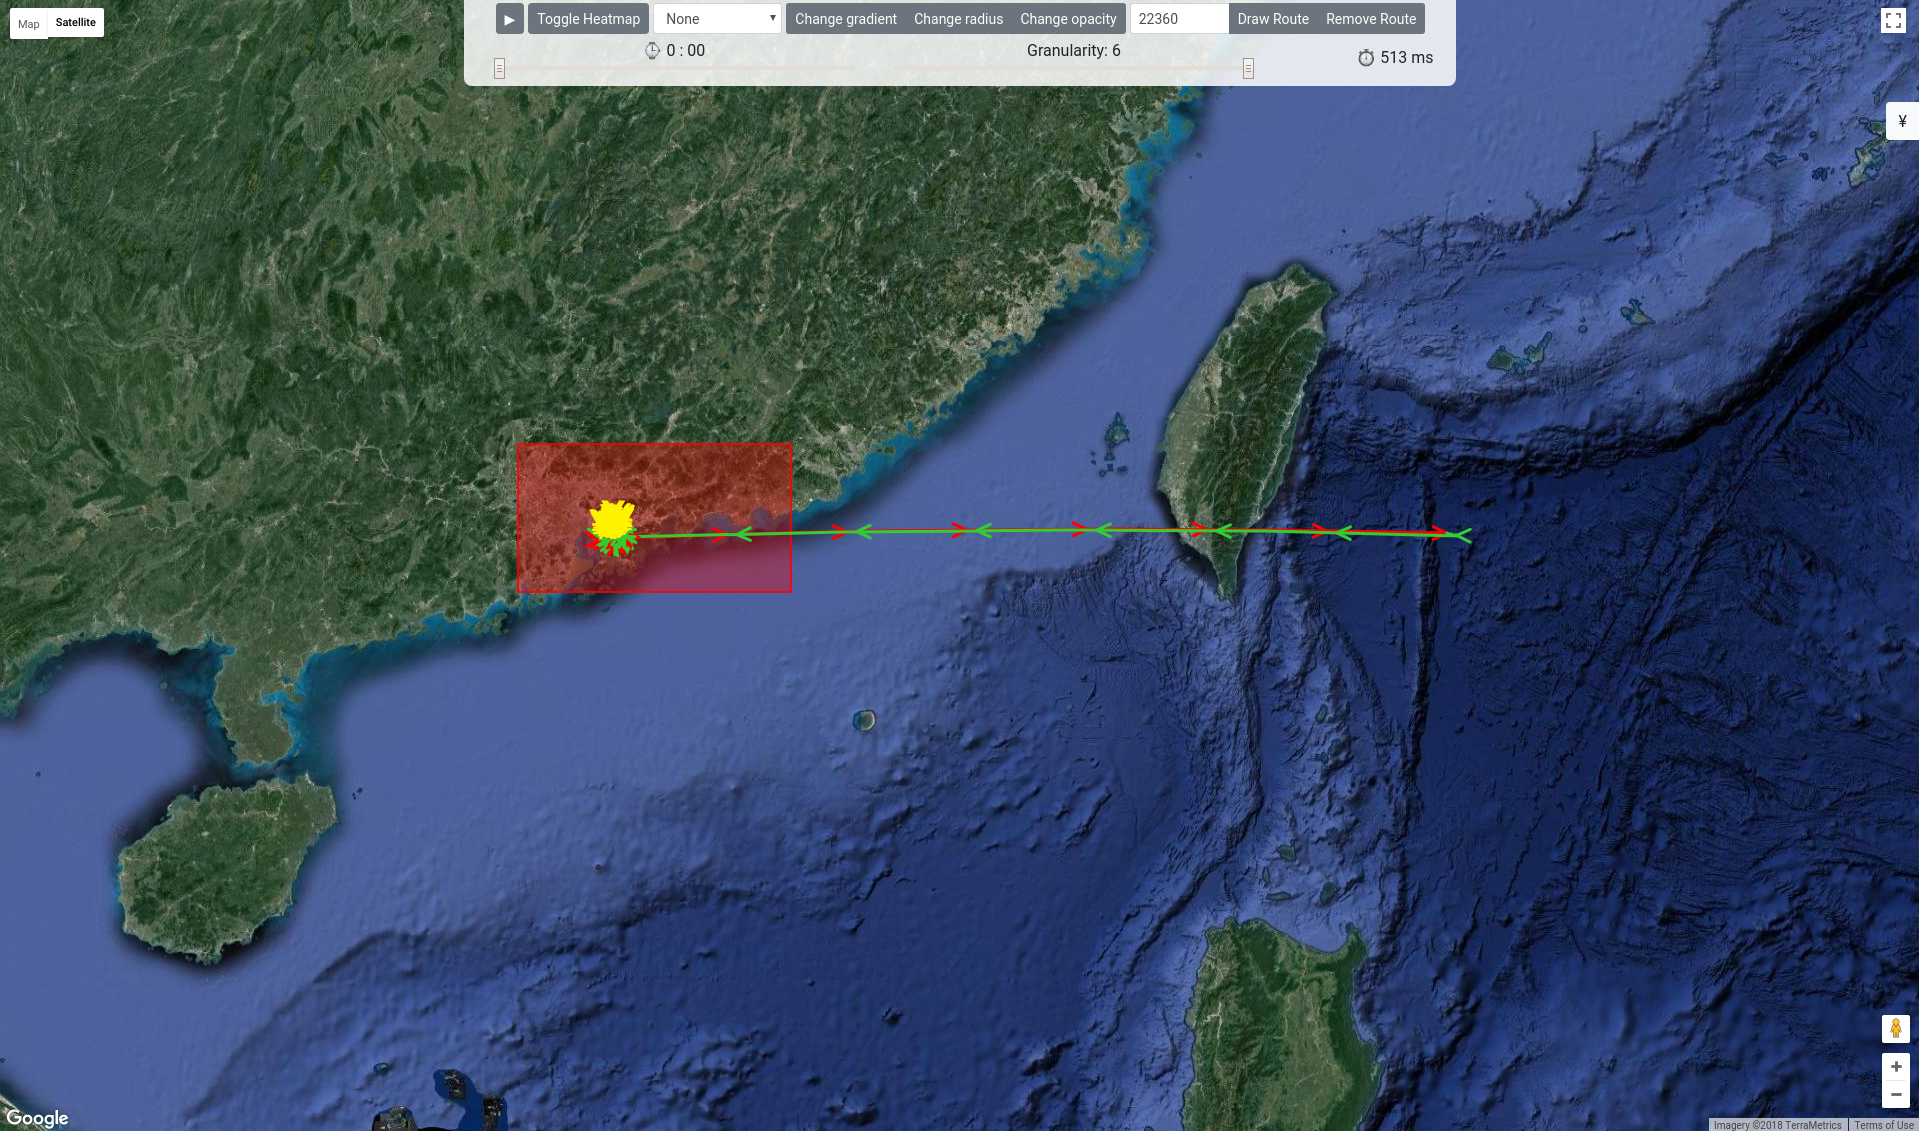
\includegraphics[width=0.5\textwidth]{img/bounding_box.png}
\caption{Bounding box and trajectory \textit{22,360} passing through the ocean}
\label{fig:bbox}
\end{figure}


\subsubsection{Small trajectories}
Some trajectories have only a few data points. The reasons for that can be of different nature. Some trajectories include only a few minutes instead of a whole day. Others have breaks lasting a couple of hours. We also noticed, that some taxis have a different time interval in terms of sending GPS locations, for example only every five minutes. In all of those cases, we delete the whole trajectory. We applied this to each taxi route having less than 500 entries.

\subsubsection{Wrong passenger status}
The status flag indicating the presence of a passenger seems to be wrong in different trajectories. We found three different scenarios and removed the whole trajetory if at least one is fulfilled. First, there are trips passing through the whole city without any passengers at all. Second, the opposite is the case: Taxis do have the same passenger for almost a day. We filtered those trajectories out by adding rules. We assume, that a taxi is supposed to have a passenger for at least two hours (not necessarily continously) and no passenger for at least one hour (also not continously) within the recorded day. In the third case, the passenger status keeps switching over time as depicted in graphic \ref{fig:passenger_status}. In order to avoid wrong calculations based on the false data, we deleted the whole trajectories.


\begin{figure}[ht]
\centering
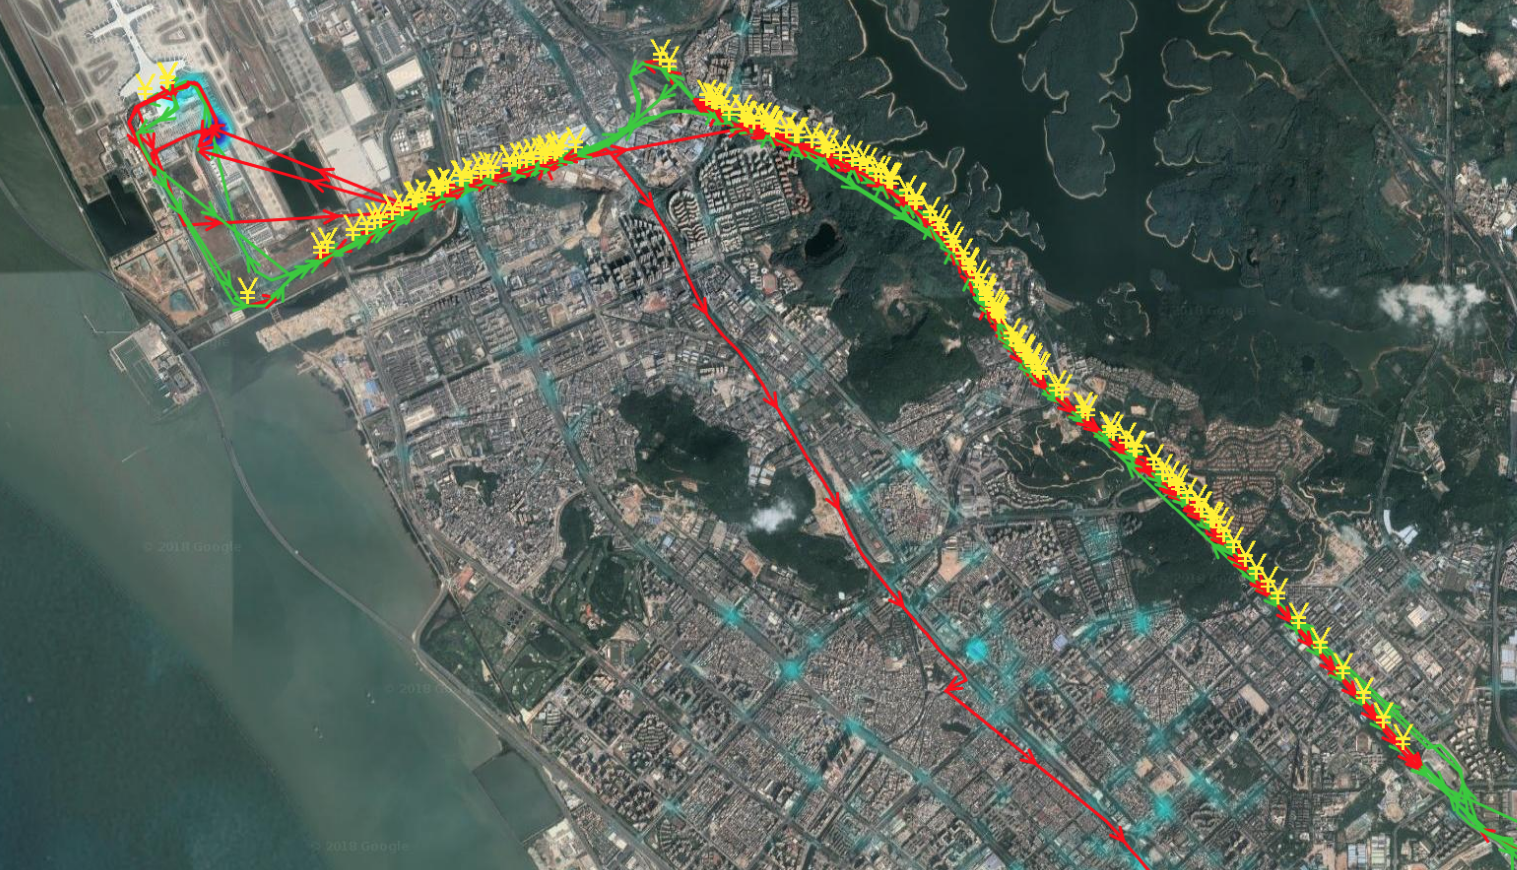
\includegraphics[width=0.5\textwidth]{img/passenger_status.png}
\caption{Passenger status changes every 30 seconds (trajectory with id \textit{27,224})}
\label{fig:passenger_status}
\end{figure}


\subsubsection{Jumps}
GPS data tends to be imprecise by nature. This results in inaccuracies as well as \quotes{jumps}. We define points that are most likely not real based on the driven speed as a jump. In order to get a better understanding of that, we depicted an example in figure \ref{fig:jump}. The green line shows an example route as it also appears in the dataset. The numbers next to the line represent the driven speed in $\frac{km}{h}$ between two points $P_i$ and $P_{i+1}$. Point $P_4$ catches the eye of the observer. The speed of more than $200\frac{km}{h}$ within the city of Shenzhen might not be even possible. To avoid such cases, we developed a Python script, that analyzes the speed between two points. If it is higher than $150\frac{km}{h}$ we take the next point into account. In our example, we calculate the speed between $P_3$ and $P_5$. Is it less than $150\frac{km}{h}$ we delete the point in between (here $P_4$). Otherwise, there is a defect that is not trivially solvable.

\begin{figure}[ht]
\centering
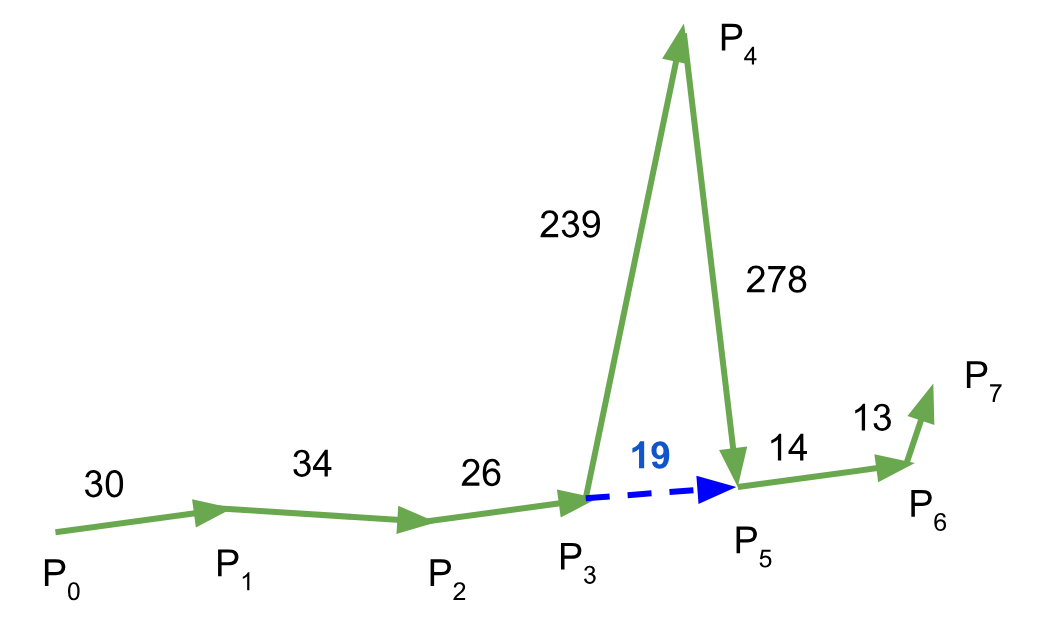
\includegraphics[width=0.5\textwidth]{img/jumps.png}
\caption{Example route containing a jump at $P_4$}
\label{fig:jump}
\end{figure}

In some cases the amount of jumps is enormously high. In such cases, we delete the whole trajectory. More specifically, this means: Every trajectory having more than 200 jumps or having more than 100 jumps that cannot be fixed are removed. One extreme example for this can be seen in figure \ref{fig:more_jumps}.

\begin{figure}[ht]
\centering
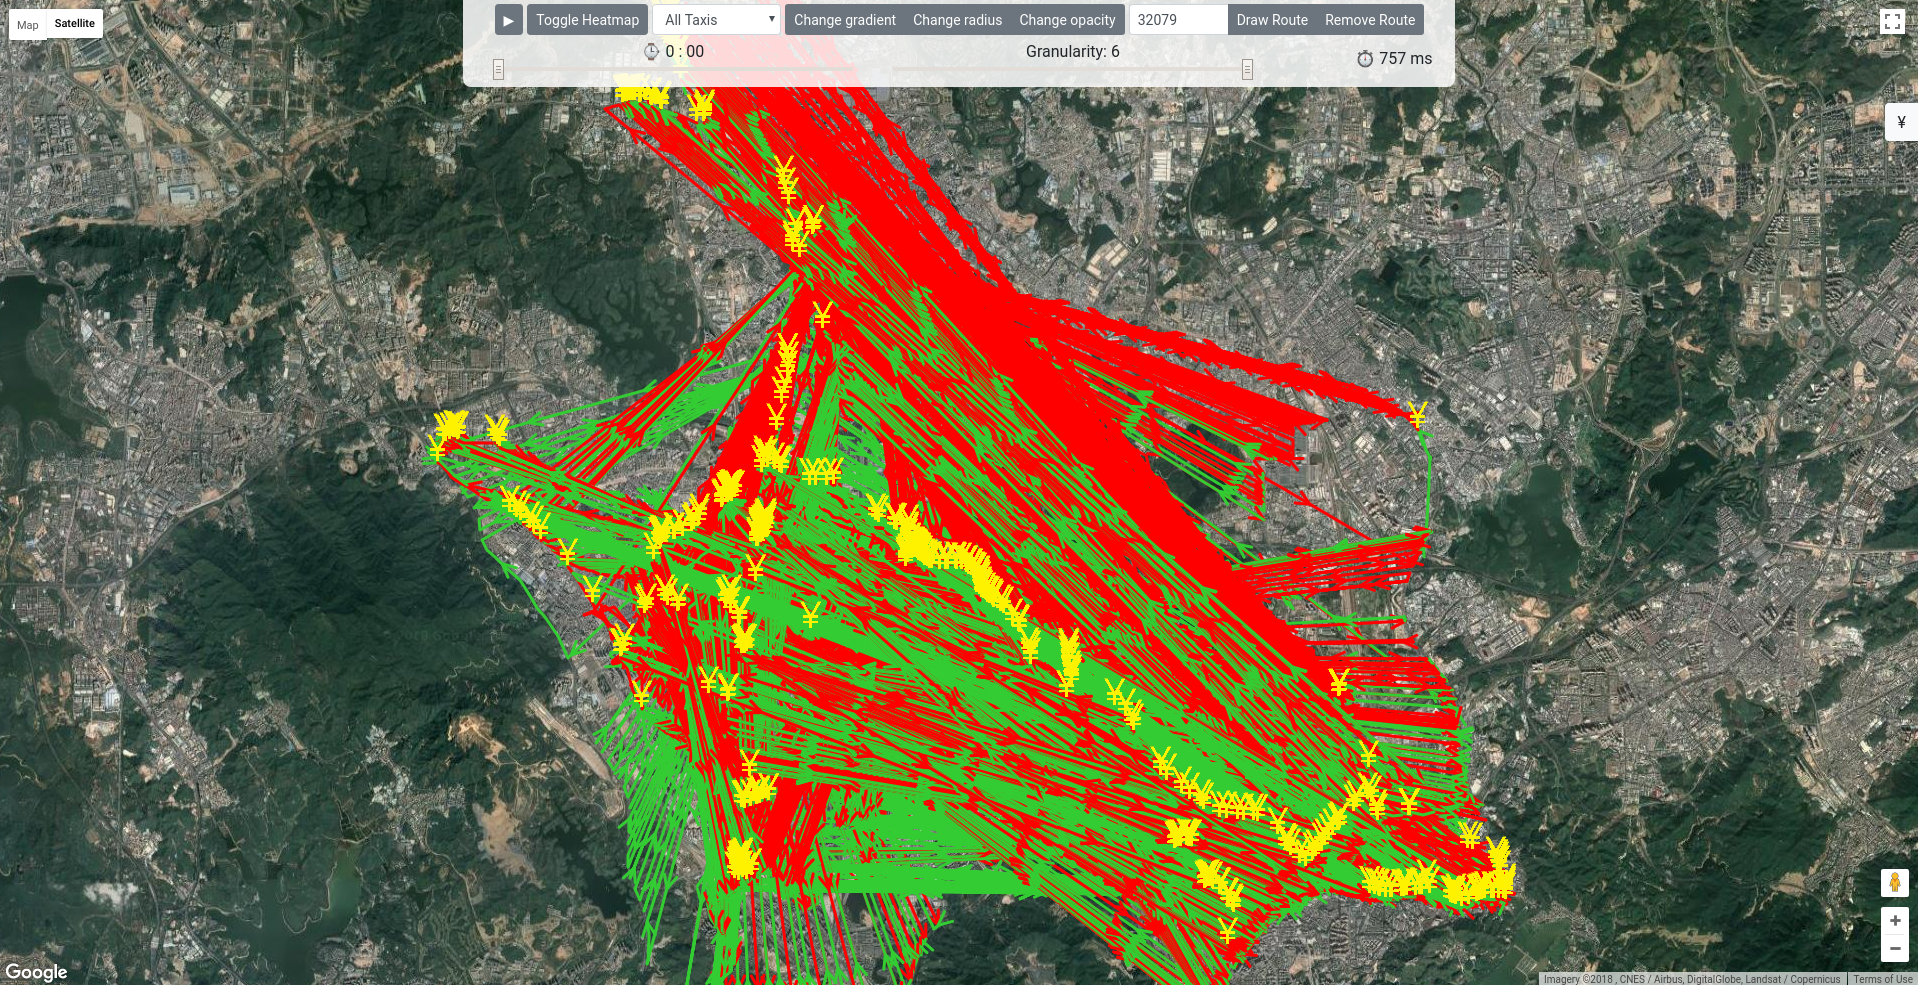
\includegraphics[width=0.5\textwidth]{img/more_jumps.png}
\caption{Trajectory \textit{} having more than 2,000 jumps}
\label{fig:more_jumps}
\end{figure}

\subsubsection{Summary: Data cleansing}
All in all we removed more than eight Million records ($\approx 18\%$) and more than 4,134 trajectories ($28\%$) due to our data cleansing rules. Most of the criteria are chosen generously to avoid deleting false positives. Additionally, there might be other aspects to improve data quality. Since this was not the focus of our work, we decided not to go further into detail.

\section{Application Prototype}

The main purpose of our application prototype is to display good performing taxis on a map. Thereby, the user can analyze how taxis get new passengers quickly. An additional task is to visualize the state at a certain time of the day. For that, we created some heatmaps (see section \ref{sec:heatmaps}).

\subsection{Taxi Profit Calculation}

The profit can be estimated with the help of the distances and the tours' start and end times. We checked the taxi fares in Shenzhen on the website Numbeo which is a database about taxi fares worldwide\footnote{\href{https://www.numbeo.com/taxi-fare/country_result.jsp?country=China}{https://www.numbeo.com/taxi-fare}}. The website says that the start of a taxi tour costs 11.00 Chinese Yuan. Then it costs 2.50 Yuan per kilometer. We have the GPS coordinates and know where a tour starts and ends. Because of that, we can calculate the driven distance and get an accurate kilometer price.

Waiting time is a component of the tour's price as well. Numbeo says that it is 48 Yuan per hour. We defined for our application that 10\% of the total time of a tour is waiting time. That is obviously not the real waiting cost for each tour, just a guess. Nevertheless, it should suffice for our prototype. A better approach would be to calculate the speed of the taxis to check if it was waiting or driving at the time.

The prices of all tours can be summed up to the profit of a taxi over the whole day. At this point we have a profit estimation for each taxi.

\subsection{Explore Profitable Taxis}

The user can see a ranking of the taxis, which had the most profit during the day. This is shown in figure \ref{fig:ranking}. The list has information about the number of tours. We also calculated the distance of each taxi while passengers were inside. This is displayed in the column \textbf{Distance km}. The list is sorted by the estimated profit which was explained in the previous section. It is displayed as the Chinese currency Yuan. When the user clicks on an entry the route for the taxi is drawn on the map.\\

\begin{figure}[ht]
\centering
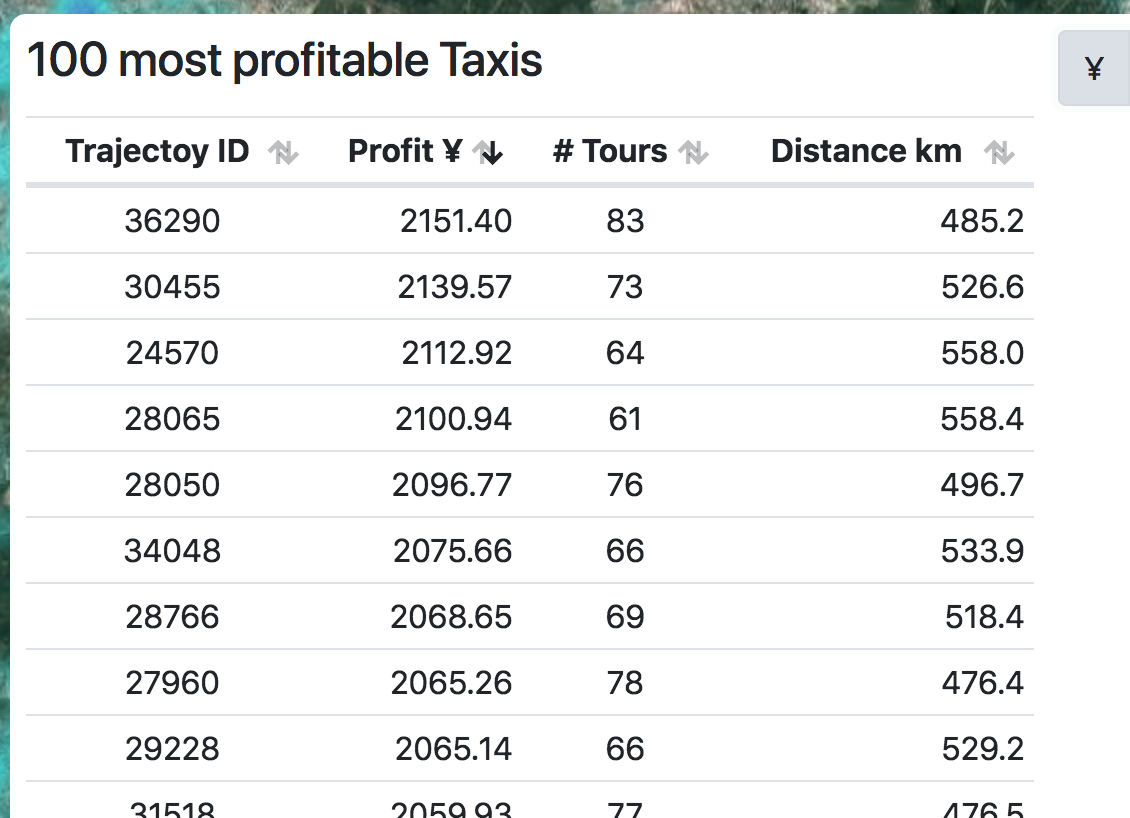
\includegraphics[width=0.5\textwidth]{img/ranking.png}
\caption{Ranking of the most profitable taxis}
\label{fig:ranking}
\end{figure}

Figure \ref{fig:single_ride} illustrates how the taxi routes are drawn. The line is red if the taxi was driven without a passenger. The line is green if it had a passenger. Arrows indicate the direction. At the end of each tour is a a Yuan symbol on which the user can click. The click lets pop up information about the tour (i.e. start time, end time, distance and the estimated profit).\\

\begin{figure}[ht]
\centering
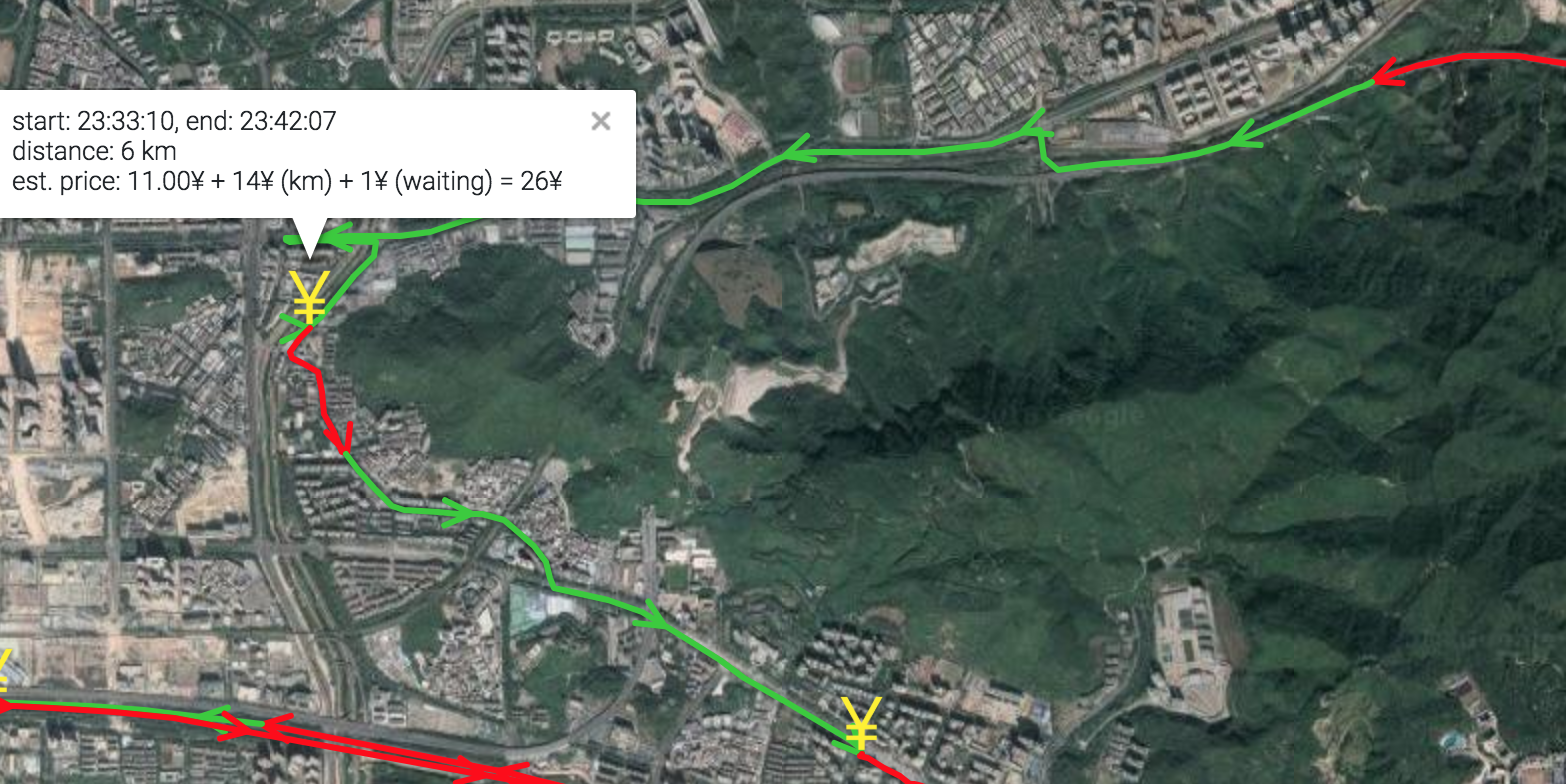
\includegraphics[width=0.5\textwidth]{img/single_ride.png}
\caption{Information about one ride}
\label{fig:single_ride}
\end{figure}

Figure \ref{fig:best_taxi} shows the route of the most profitable taxi (ID \textit{36290} in figure \ref{fig:ranking}). You can see that this taxi had the most tours in one area. The taxi had 83 tours during the day. These tours sum up to a distance of 482 kilometers. The red lines are often very short.

\begin{figure}[ht]
\centering
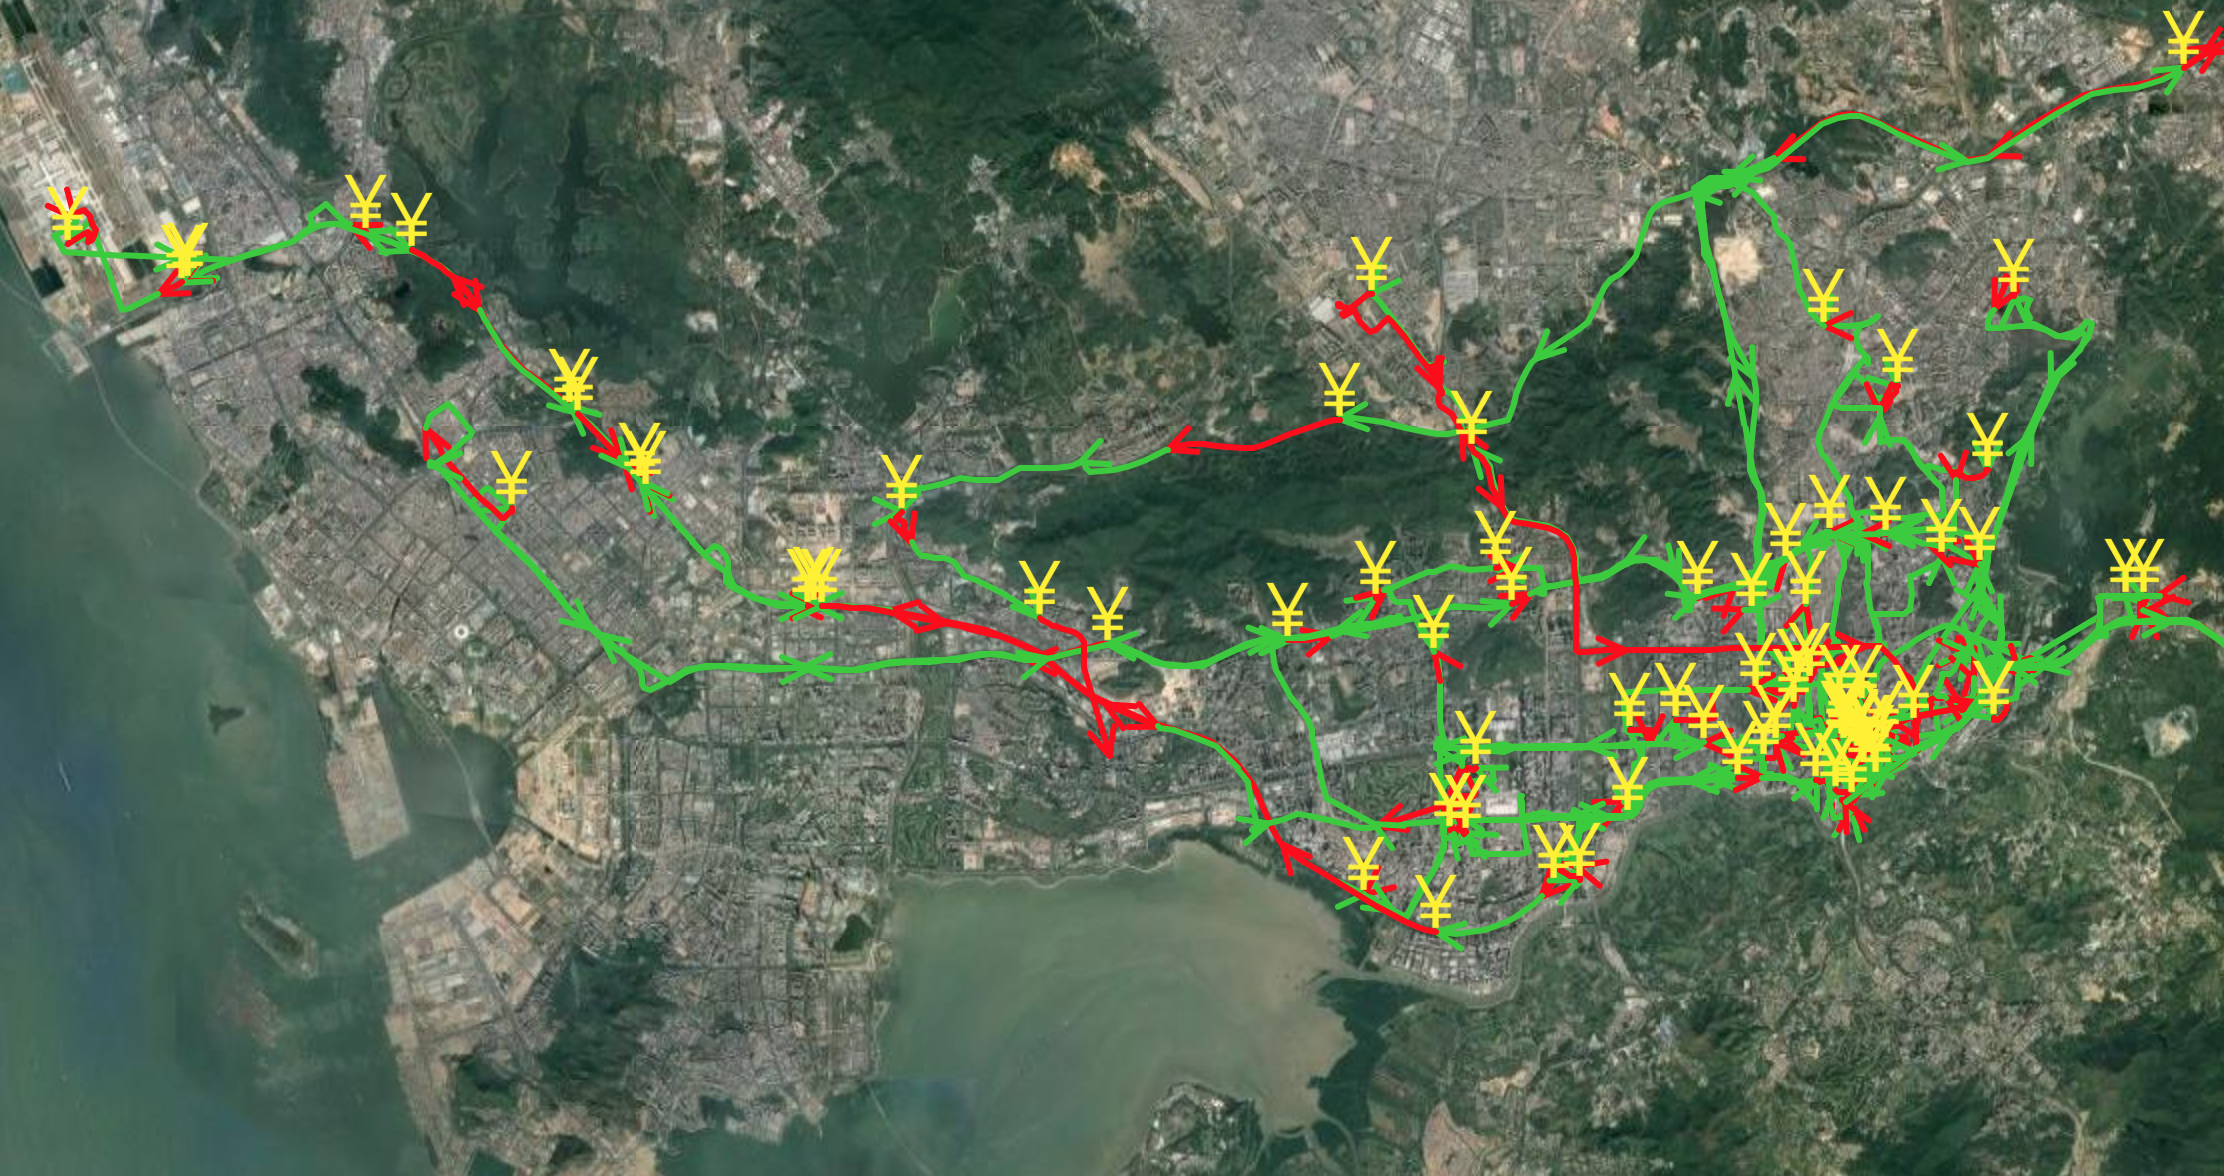
\includegraphics[width=0.5\textwidth]{img/best_taxi.png}
\caption{Entire taxi route}
\label{fig:best_taxi}
\end{figure}

\subsection{Heatmaps}
\label{sec:heatmaps}

The application has a taxi density heatmap (see figure \ref{fig:density}). The areas, which have many taxis at the given time, are colored red. Areas with less taxis are colored blue. The user interface has a time slider. When changing the time from 3:00 PM to another time, the map would refresh. In the top left corner is a play button. With the play function, the map continually updates to the next time interval. Thus, the user can observe how the taxi density changes over time.

\begin{figure}[ht]
\centering
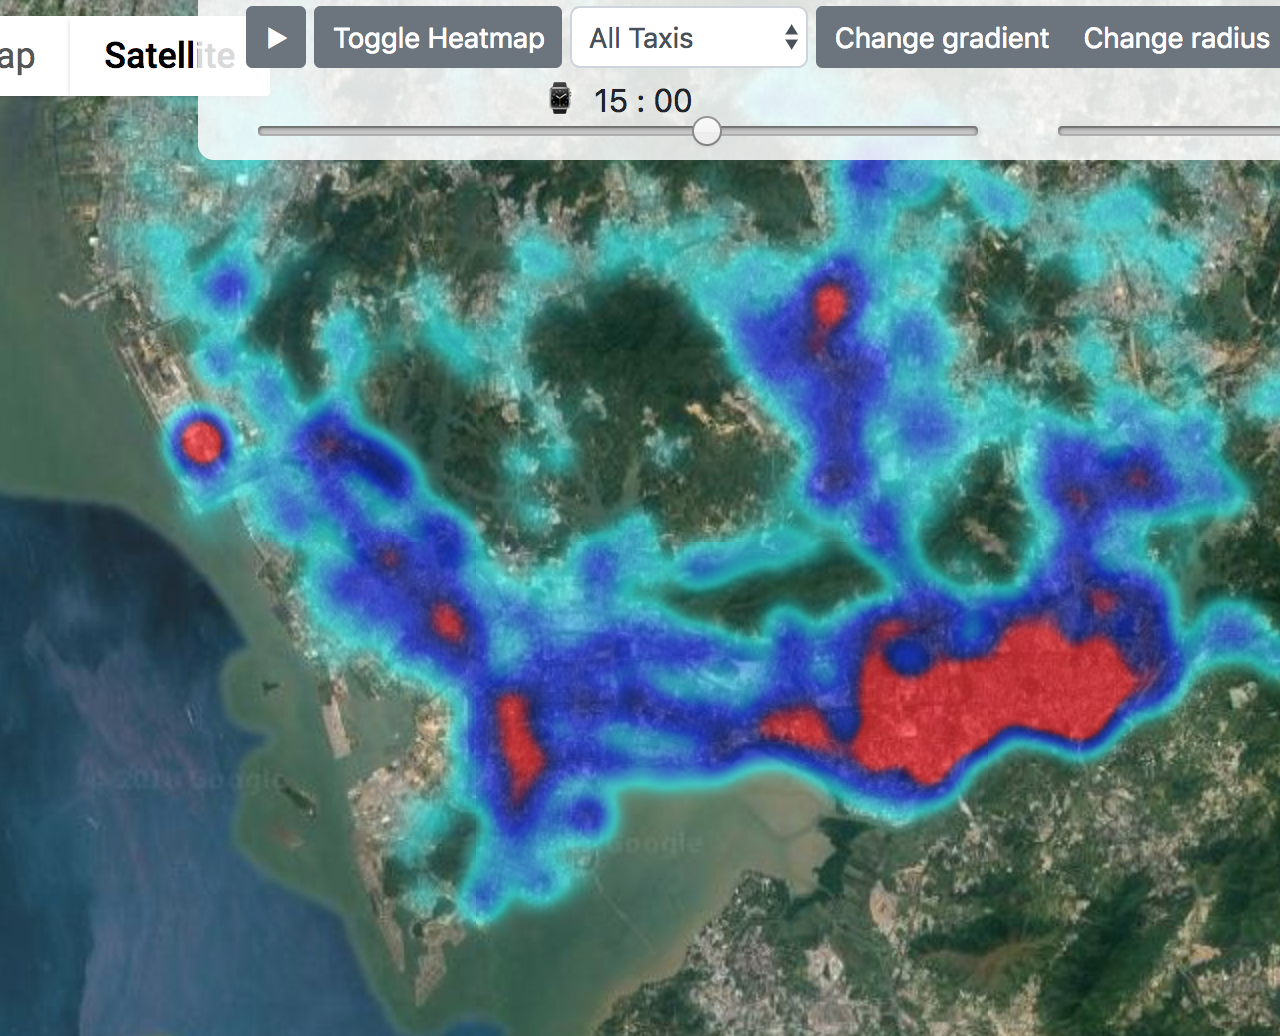
\includegraphics[width=0.5\textwidth]{img/density.png}
\caption{Taxi density heatmap}
\label{fig:density}
\end{figure}

The heatmap can visualize two other things. One of these is the number of picked up passengers. The other one is the number of dropped passengers. The user interface has a dropdown menu to let the user select which heatmap is displayed.

\subsection{System Architecture}

This section is about our architecture. Figure \ref{fig:architecture} is a FMC (Fundamental Modeling Concepts) diagram. Our architecture can be divided into the three components frontend, backend and database. We have a web application. Hence, it runs in a browser. We are using the Google Maps API. In our frontend, we are using HTML5 and Javascript.\\

\begin{figure}[ht]
\centering
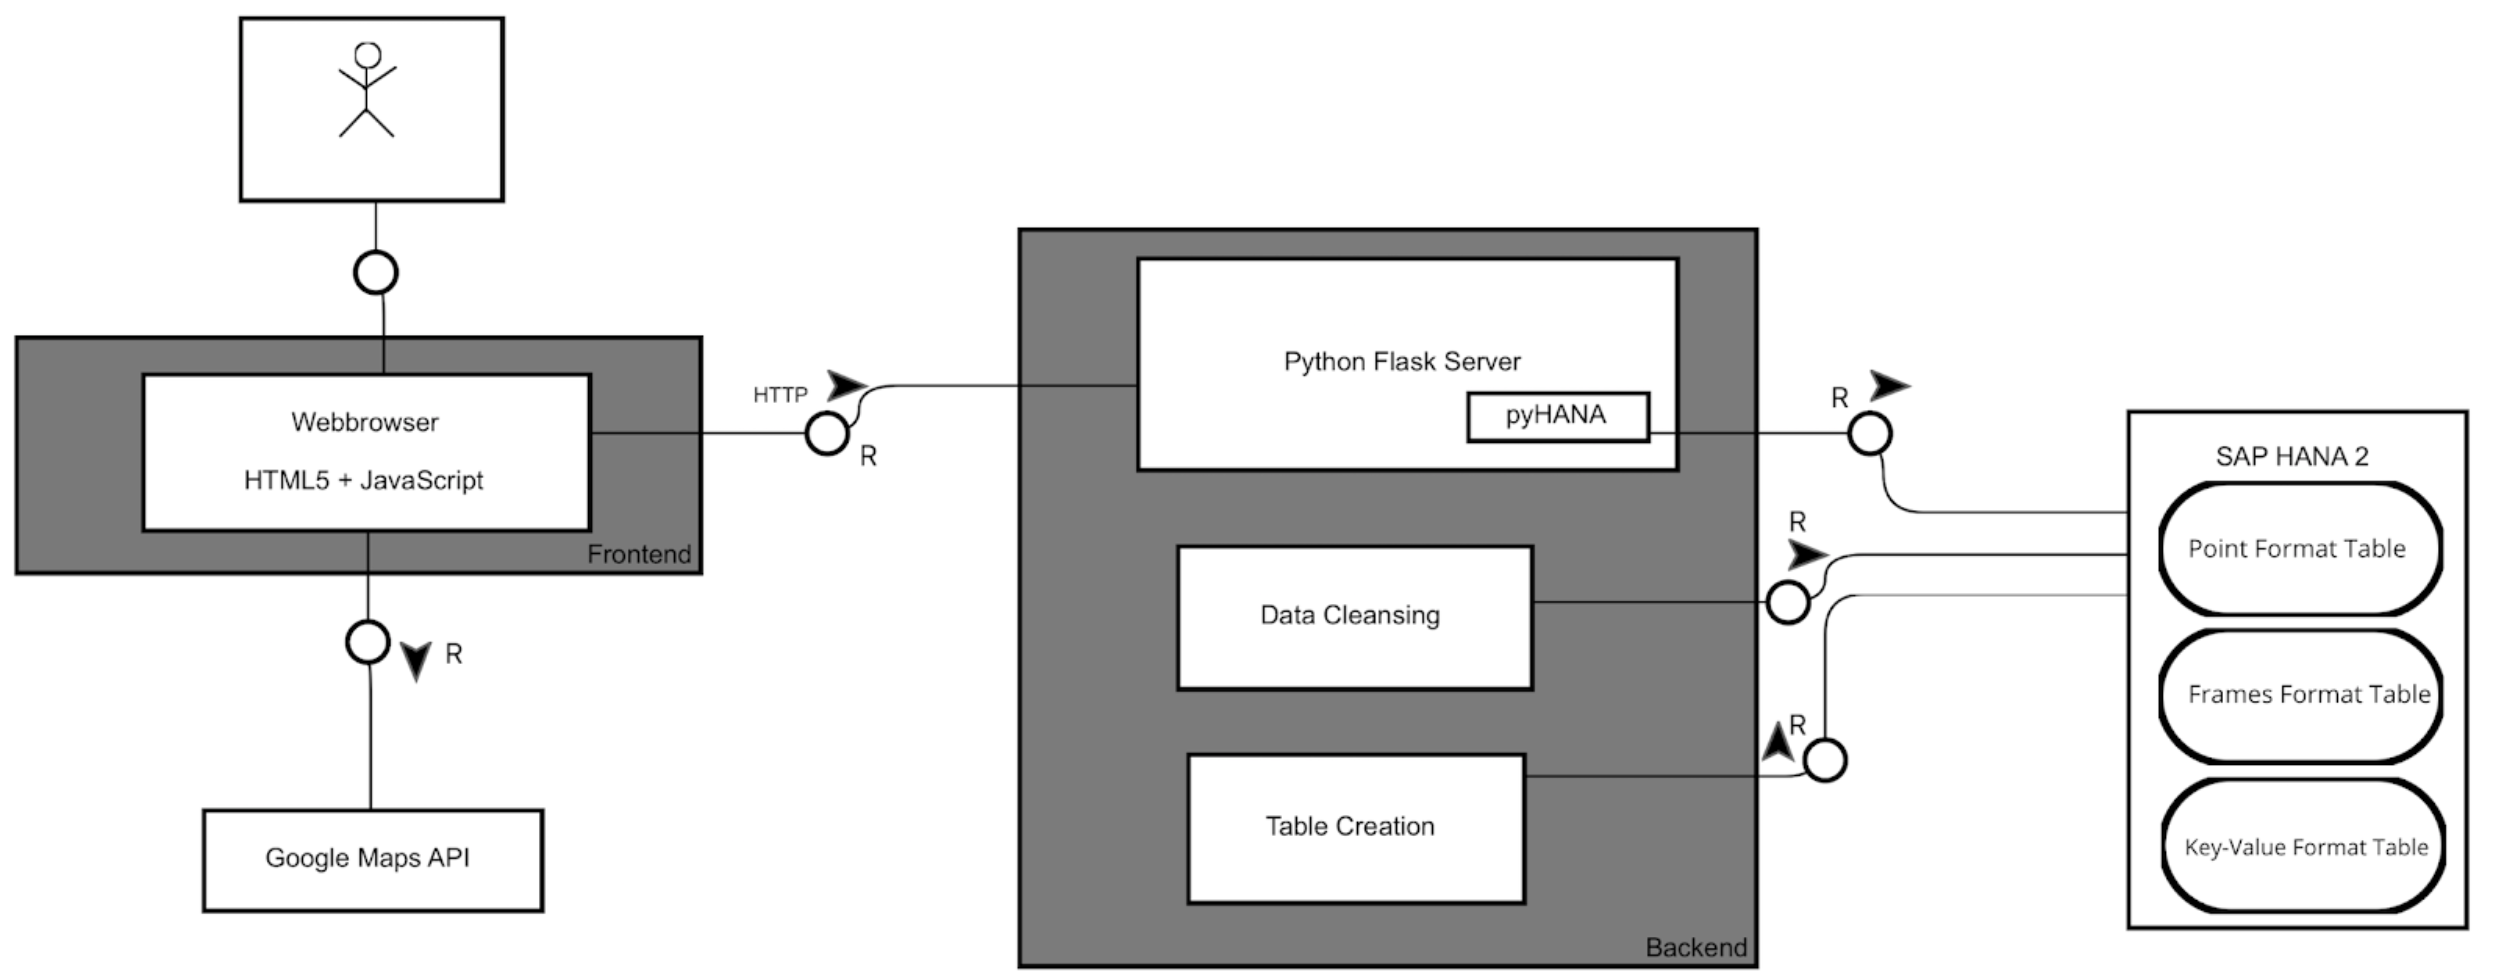
\includegraphics[width=0.5\textwidth]{img/architecture.png}
\caption{System architecture}
\label{fig:architecture}
\end{figure}

The backend essentially has a REST API which is written in Python and uses the Flask framework. It serves the static HTML and Javascript files, as well as redirecting requests to the database. The backend also has a few python scripts that are used to create tables and for the data cleansing.

The database, which we are using, is SAP HANA. It stores all of the data in different table formats. The table formats are elaborated in section \ref{sec:data_layouts}. The database has some procedures that can be executed to answer non trivial data requests (e.g. to get the calculated profits). 

The communication between the backend and the database in managed via pyHANA\footnote{\href{https://github.com/hpi-epic/pyHANA}{https://github.com/hpi-epic/pyHANA}}. pyHANA is a Python client for SAP HANA.


\section{Data Layouts}
\label{sec:data_layouts}
A crucial factor for SQL query performance is the way the data is stored. Therefore, we tried out three different layouts which we want to present in this section.
\subsection{Sample point format}
The sample point format is similar to the way the data is stored in the CSV-file. Each GPS sample corresponds to one row within the database. Furthermore, each attribute is stored in one column without any manual encoding.

The layout has three major advantages. First, the data can be accessed directly. There is no need for further calculation or modification in order to obtain a specific value. Second, the data stays as it is. Since there is no normalization, we always have the full dataset in hand. Additionally, the amenities of column store can be exploited. SAP Hana supports various internal compression types in order to reduce the amount of memory used. Less data has to be loaded from memory, which leads to a higher throughput and faster query execution times.

The whole table consumes about 498 MB of main memory after applying the data cleansing rules. We prefer the column store over the row store in this case.

\subsection{Frame format}
Another way of storing the information is the frame format. This approach is presented by Wang et al.~\cite{wang} The main idea behind this layout is splitting the sample sample points into frame groups of a fixed length with a fixed frequency of data points. We decided to use a frame size of 30 seconds and a frame group size of one hour as described in the paper by Wang et al.

In order to keep the right order of the data points after splitting a trajetory into multiple frame groups a frame group identifier (\textit{FGCID}) has to be introduced (cf. figure \ref{fig:frame_format}). The starting point's GPS location of a frame group is stored in the column \textit{IFX} (longitude) and \textit{IFX} (latitude). In order to save memory the subsequent points are encoded as the deltas of the coordinates. The columns are named \textit{PF0X, PF0Y, PF1X, PF1Y, ..., PF119X, PF119Y}. Hence the frame format table consists of 244 columns.

\begin{figure}[ht]
\centering
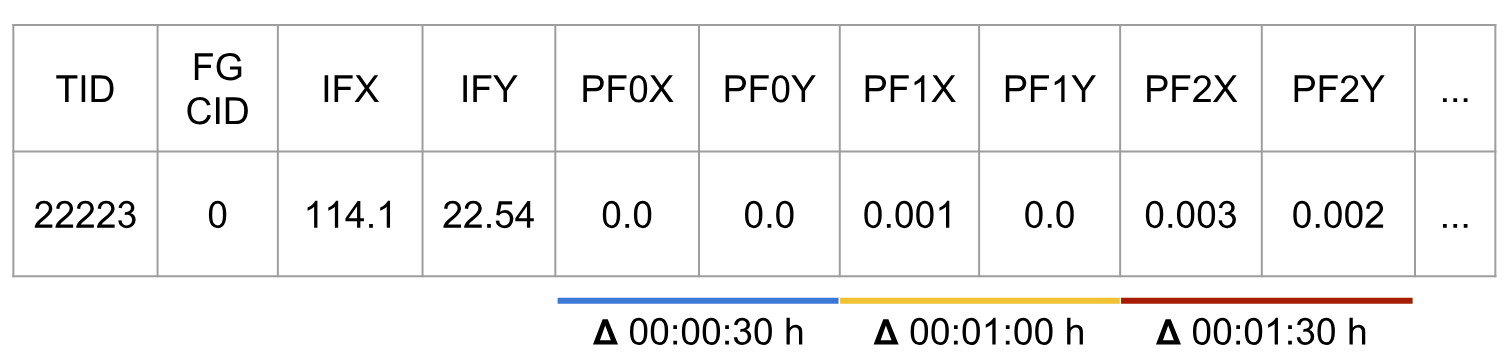
\includegraphics[width=0.48\textwidth]{img/frame_format.png}
\caption{Information stored in frame format}
\label{fig:frame_format}
\end{figure}

This approach avoids using timestamps, which is a major advantage in term of memory consumption. Also querying a time series is supposed to be faster compared to the frame format. However, the different positions within the frames have to be calculated, which can be a tedious thing. Due to the use of frames the data is normalized by time on the one hand. On the other hand, there is a loss of information. Furthermore, there could be the possibility of missing points. In this case, Wang et al.~\cite{wang} calculate those points via SED distance. We refrain from that. The overall frame format table with a framegroup size of ten minutes and a frame size of 15 seconds consumes circa 441 MB of main memory, when stored in column layout. In total, there are more than 2 million rows.

\subsection{Key-Value format}

A third storage layout we evaluated is the key-value format. Therefore, we decided to encode a whole trajectory as an array of arrays containing longitude, latitude and the corresponding timestamp. Since an array cannot be stored in the SAP Hana database, we take its string representation and filed it in a column of data type \textit{NCLOB}. An example can be found in code listing \ref{lst:json}. We do not normalize by time. Hence, there is no loss in terms of GPS data. Besides this information, there are the trajectory identifier, start and end time and the mininum bounding rectangle present in the table. In total, there are 10,594 (equivalent to the amount of trajectories after data cleansing) consuming about 650 MB of main memory in column store.

\lstset{language=json}
\begin{minipage}{0.45\textwidth}
\begin{lstlisting}[frame=single, firstnumber=1, caption=Key-Value format example entry,label=lst:json]
"[
    [
        "0001-01-01 00:00:03",
        22.512432,
        113.913933
    ],
    [
        "0001-01-01 00:00:58",
        22.5163,
        113.917068
    ],
    ...
]"
\end{lstlisting}
\end{minipage}


\subsection{Optimizations}


this layout is splitting the sample sample points into frame groups of a fixed length with a fixed frequency of data points. We decided to use a frame size of 15 seconds, since this is the median frequency the data was recorded (see section \ref{sec:ds}). Furthermore, we use a frame group size of ten minutes.


\section{Benchmark Results}

\section{Conclusion}

% \bibliographystyle{ACM-Reference-Format}
\bibliographystyle{plain}
\bibliography{references}

\end{document}
